\documentclass[aspectratio=169]{beamer}
\usepackage[utf8]{inputenc}
\usepackage{graphicx}
\usepackage{hyperref}

\usetheme{Madrid}
\usecolortheme{default}

\title{Modelos Visión-Lenguaje (VLMs)}
\subtitle{Large vision-language models}
\author[Juan Irving Vasquez \textit{jivg.org}] % (optional)
{Juan Irving Vásquez\inst{1}}
\date{\today}
\titlegraphic{
\includegraphics[width=2cm]{ipn-cidetec}}

\institute[IPN] % (optional)
{
  \inst{1}%
  Centro de Innovación y Desarrollo Tecnológico en Cómputo\\
  Instituto Politécnico Nacional
}

\begin{document}

% --- PORTADA ---
\begin{frame}
    \titlepage
\end{frame}

% --- INTRODUCCIÓN ---
\begin{frame}{¿Qué son los Modelos Visión-Lenguaje?}
\begin{figure}
    \centering
    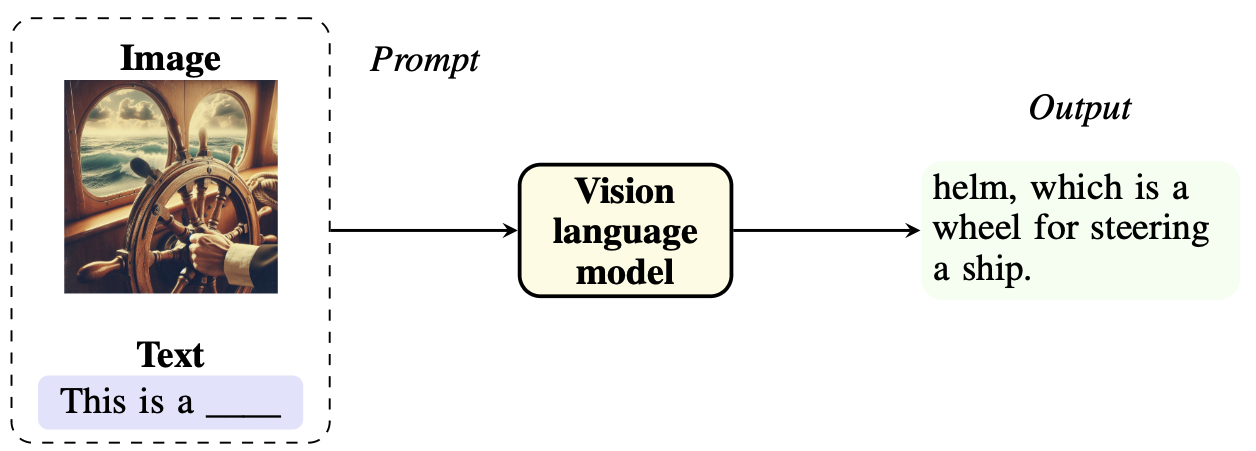
\includegraphics[width=0.6\linewidth]{vlm1.png}
    %\caption{Enter Caption}
    %\label{fig:placeholder}
\end{figure}
    \begin{itemize}
        \item Los \textbf{Modelos Visión-Lenguaje (VLMs)} combinan la visión por computadora y el procesamiento de lenguaje natural (NLP) en un solo sistema multimodal. 
        \item Integran un \textit{codificador visual} y un \textit{modelo de lenguaje grande (LLM)}, permitiendo razonar sobre imágenes, videos y texto simultáneamente.
        \item Ejemplos de tareas: generar subtítulos de imágenes, responder preguntas visuales o buscar imágenes mediante descripciones textuales.
    \end{itemize}
\end{frame}

% --- DIAGRAMA GENERAL ---
\begin{frame}{Esquema general}
    \begin{figure}
        \centering
        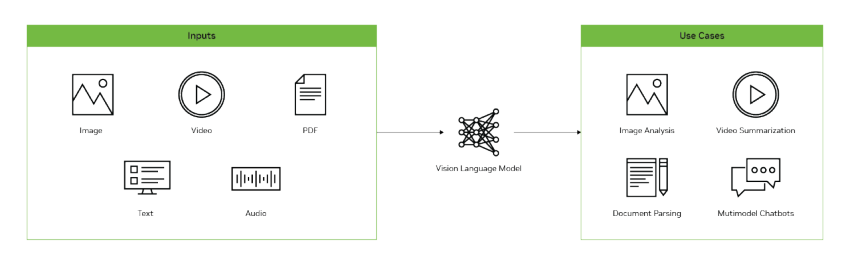
\includegraphics[width=\linewidth]{metropolis-iva-diagram-vlm-glossary-ces25-3576177-r1--1-.png}
        \caption{Ejemplo de flujo multimodal entre visión y lenguaje.}
    \end{figure}
\end{frame}

% --- IMPORTANCIA ---
\begin{frame}{Importancia de los VLMs}
    \begin{itemize}
        \item Superan las limitaciones de los modelos tradicionales de visión, al no restringirse a un conjunto fijo de clases o tareas.
        \item Gracias a su entrenamiento en grandes colecciones de pares imagen-texto, pueden aprender instrucciones en lenguaje natural y adaptarse a nuevas tareas.
        \item Habilitan aplicaciones de \textbf{IA generativa multimodal}, integrando texto, imagen, audio y video.
    \end{itemize}
\end{frame}


% --- ARQUITECTURA (COMBINADA) ---
\begin{frame}{Arquitectura de los VLMs}
\begin{columns}[T,onlytextwidth]

% --- Columna Izquierda: Texto ---
\begin{column}{0.45\textwidth}
    \begin{itemize}
        \item Tres bloques principales:
        \begin{enumerate}
            \item \textbf{Codificador de visión:} transforma imágenes o video en embeddings.
            \item \textbf{Fusor o proyector:} alinea los espacios de visión y lenguaje en un mismo dominio semántico.
            \item \textbf{Modelo de lenguaje grande (LLM):} interpreta o genera texto a partir de la información visual.
        \end{enumerate}
        \item Generalmente se basan en arquitecturas tipo \textit{Transformers}, como \textbf{CLIP} o \textbf{ViT}.
        \item La integración de estos módulos permite razonar de forma multimodal y generar respuestas contextuales.
    \end{itemize}
\end{column}

% --- Columna Derecha: Imagen ---
\begin{column}{0.45\textwidth}
    \begin{figure}
        \centering
        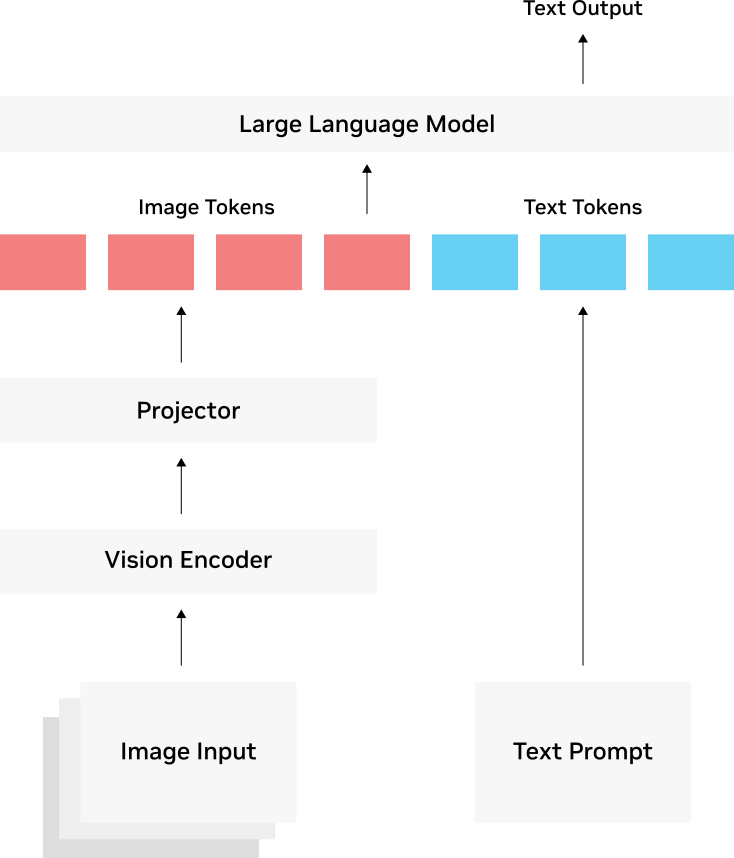
\includegraphics[width=0.7\textwidth]{vlm-architecture-diagram.png}
        \caption{Arquitectura típica de un modelo Visión-Lenguaje.}
    \end{figure}
\end{column}

\end{columns}
\end{frame}



% --- ENTRENAMIENTO ---
\begin{frame}{Entrenamiento de los VLMs}
    \begin{itemize}
        \item Los VLMs se entrenan mediante diversas estrategias:
        \begin{enumerate}
            \item \textbf{Aprendizaje contrastivo:} alinea embeddings de imagen y texto (ej. CLIP).
            \item \textbf{Enmascaramiento:} predice partes ocultas en texto o imagen.
            \item \textbf{Entrenamiento generativo:} produce texto desde imágenes o viceversa.
        \end{enumerate}
        \item Generalmente combinan modelos preentrenados de visión y lenguaje antes de un ajuste fino (\textit{fine-tuning}) en datos multimodales específicos.
    \end{itemize}
\end{frame}

\begin{frame}{Diagrama del Proceso de Entrenamiento}
    \begin{figure}
        \centering
        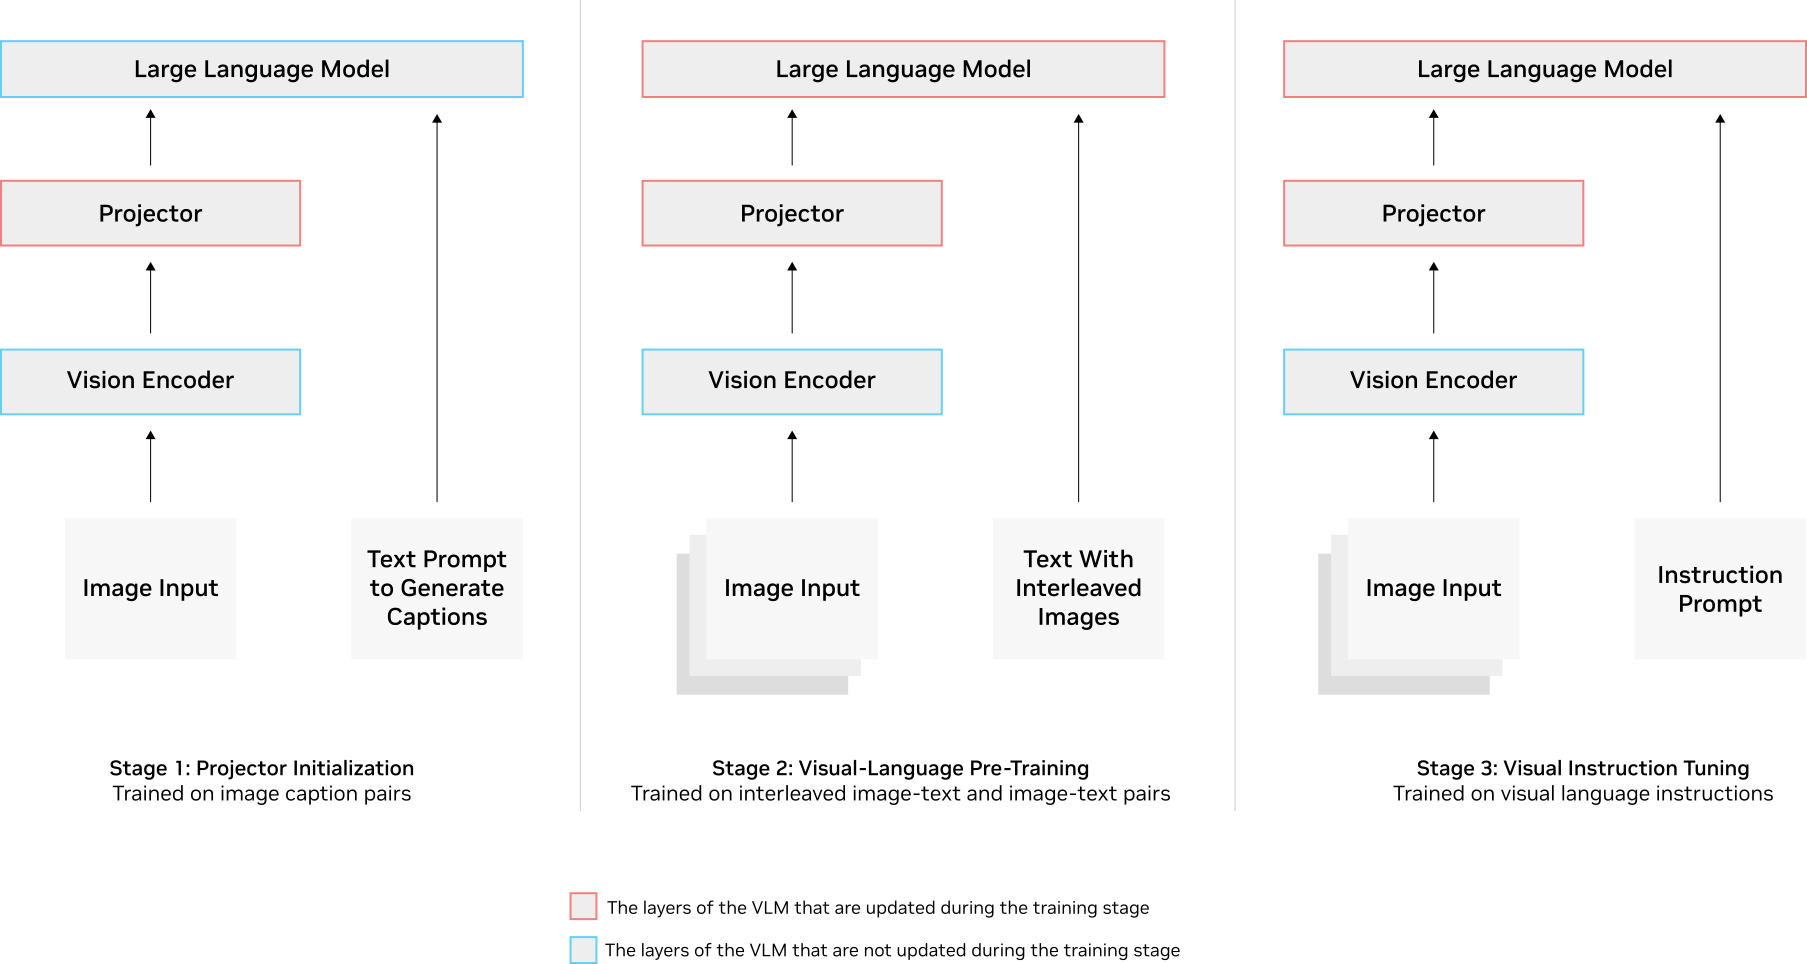
\includegraphics[width=0.9\linewidth]{vlm-training-process-diagram.png}
    \end{figure}
\end{frame}

% --- MODELOS REPRESENTATIVOS ---
\begin{frame}{Modelos Representativos}
    \begin{itemize}
        \item \textbf{CLIP (OpenAI):} pionero en aprendizaje contrastivo imagen-texto.
        \item \textbf{GPT-4o (OpenAI):} modelo multimodal capaz de procesar texto, imagen y audio.
        \item \textbf{Gemini 2.0 Flash (Google):} integración completa entre texto, imagen, audio y video.
        \item \textbf{Llama 3.2 (Meta):} modelo abierto con entrada de visión y texto.
        \item \textbf{NVLM (NVIDIA)} y \textbf{Qwen 2.5-VL (Alibaba)}: especializados en imágenes de alta resolución y video de larga duración.
    \end{itemize}
\end{frame}

% --- EVALUACIÓN ---
\begin{frame}{Evaluación de VLMs}
    \begin{itemize}
        \item Se evalúan mediante pruebas multimodales que miden razonamiento, comprensión visual y precisión textual:
        \begin{enumerate}
            \item \textbf{MMBench, MMMU, MM-Vet}: razonamiento general.
            \item \textbf{OCRBench, MathVista}: comprensión de texto y símbolos en imágenes.
            \item \textbf{VQA}: respuestas a preguntas visuales.
        \end{enumerate}
        \item La evaluación busca medir tanto la precisión como la capacidad de generalización y razonamiento multimodal.
    \end{itemize}
\end{frame}

\begin{frame}{Ejemplo de evaluación}
\begin{figure}
    \centering
    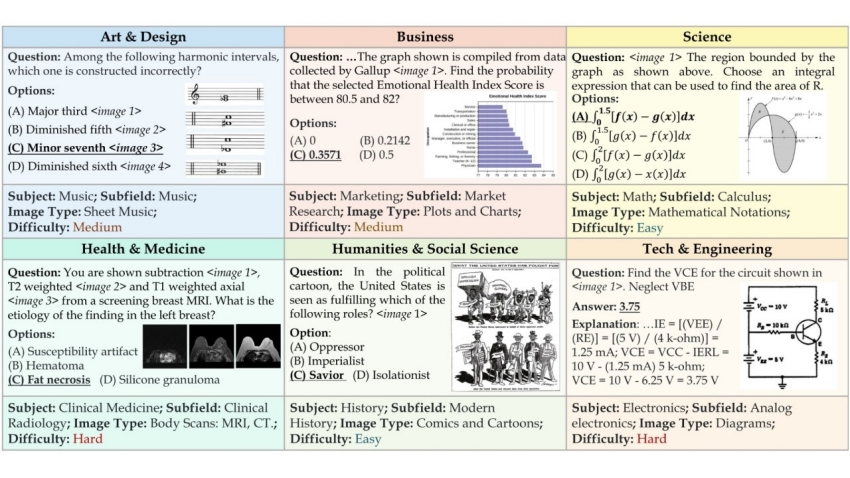
\includegraphics[width=0.8\linewidth]{vlm-mmmu-ari.jpeg}
\end{figure}
\end{frame}

% --- APLICACIONES ---
\begin{frame}{Aplicaciones de los VLMs}
    \begin{itemize}
        \item \textbf{Generación de descripciones} de imágenes o videos.
        \item \textbf{Búsqueda visual semántica}: encontrar imágenes a partir de texto.
        \item \textbf{Segmentación y detección de objetos} con explicación textual.
        \item \textbf{Respuesta a preguntas visuales (VQA)}.
        \item \textbf{Diseño asistido y generación de imágenes} (text-to-image).
        \item Usos en medicina, robótica, educación, arte y sistemas de monitoreo ambiental.
    \end{itemize}
\end{frame}

\begin{frame}{Aplicaciones en el mundo real}
 \begin{figure}
     \centering
     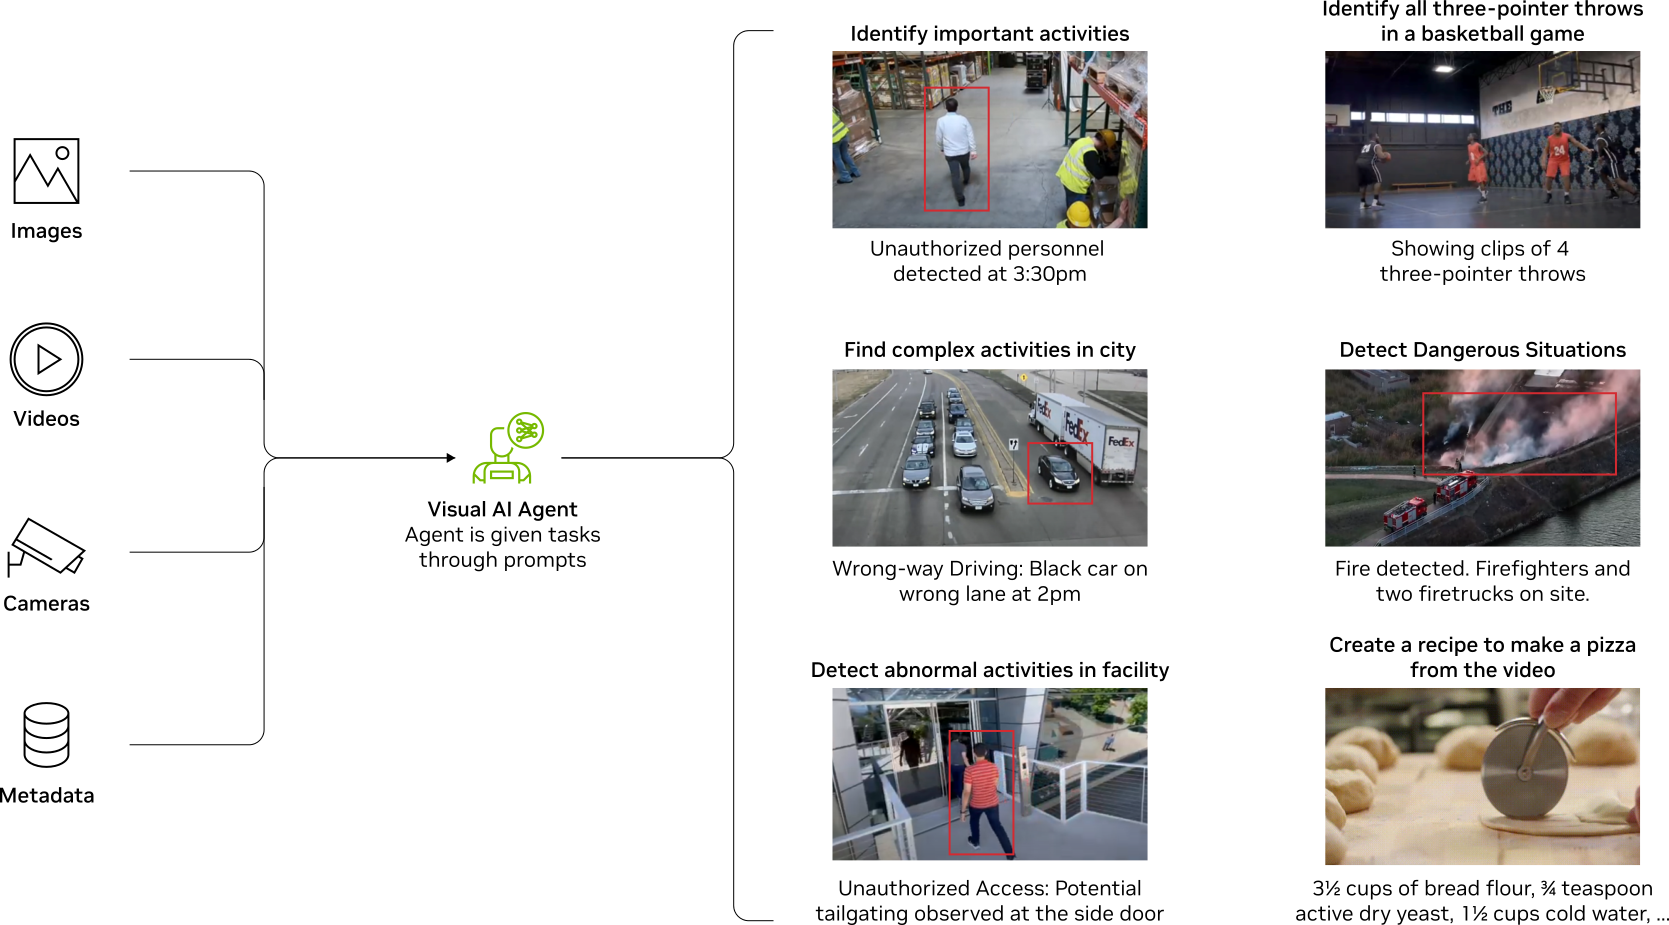
\includegraphics[width=0.8\linewidth]{vlm-real-world-diagram.png}
 \end{figure}
\end{frame}

% --- DESAFÍOS ---
\begin{frame}{Desafíos y Riesgos}
    \begin{itemize}
        \item \textbf{Sesgos de datos:} los modelos pueden reflejar prejuicios presentes en los conjuntos de entrenamiento.
        \item \textbf{Costos computacionales elevados} para entrenamiento y despliegue.
        \item \textbf{Generalización limitada} en escenarios no vistos o de dominio distinto.
        \item \textbf{Alucinaciones}: generación de descripciones falsas o incorrectas.
        \item \textbf{Gobernanza y ética}: necesidad de regulación, validación y control humano.
    \end{itemize}
\end{frame}

% --- CONCLUSIÓN ---
\begin{frame}{Conclusiones}
    \begin{itemize}
        \item Los VLMs integran comprensión visual y lingüística en un solo sistema, habilitando una nueva generación de aplicaciones multimodales.
        \item Representan un paso hacia \textbf{IA generalista}, capaz de razonar sobre múltiples modalidades.
        \item Su futuro depende de avances en alineación, ética, eficiencia y robustez.
    \end{itemize}
\end{frame}

% --- REFERENCIAS ---
\begin{frame}{Referencias}
    \begin{thebibliography}{9}
        \bibitem{ibm_vlm} IBM Think (2025). \textit{What are Vision-Language Models?} Disponible en: \url{https://www.ibm.com/think/topics/vision-language-models}
        \bibitem{nvidia_glossary} NVIDIA Glossary (2024). \textit{What are Vision-Language Models?} \url{https://www.nvidia.com/en-us/glossary/vision-language-models/}
    \end{thebibliography}
\end{frame}

\end{document}
